\subsection{Vorgehen}
\frame{
\frametitle{Unser Beispiel mit MapReduce}
\begin{itemize}
\item
Eigenwert Problem lösen
\item
Google Page Rank als Ziel
\item
Aufteilen und zusammenfügen grosser Matrizen
\item
Wir verwenden die im Unterricht bearbeitete Potenzmethode
\end{itemize}
}
\frame{
  \frametitle{Potenzmethode}

$$
\begin{bmatrix}
u_1 \\
u_2 \\
u_3 \\
u_4 \\
u_5 \\
u_6 \\
u_7 \\
u_8 \\
\end{bmatrix}
=
\begin{bmatrix}
\frac{2}{4} & \frac{1}{4} & 0 & 0 & 0 & 0 & 0 & 0 \\
\frac{2}{4} & \frac{1}{4} & \frac{1}{3} & 0 & 0 & 0 & 0 & 0 \\
0 & \frac{1}{2} & \frac{1}{3} & \frac{1}{5} & 0 & 0 & 0 & 0 \\
0 & 0 & \frac{1}{3} & \frac{3}{5} & \frac{1}{3} & 0 & 0 & 0 \\
0 & 0 & 0 & \frac{1}{5} & \frac{1}{3} & \frac{1}{4} & 0 & 0 \\
0 & 0 & 0 & 0 & \frac{1}{3} & \frac{1}{2} & \frac{2}{6} & 0 \\
0 & 0 & 0 & 0 & 0 & \frac{1}{4} & \frac{3}{6} & \frac{3}{5}\\
0 & 0 & 0 & 0 & 0 & 0 & \frac{1}{6} & \frac{2}{5} \\
\end{bmatrix}
\cdot
\begin{bmatrix}
u_1 \\
u_2 \\
u_3 \\
u_4 \\
u_5 \\
u_6 \\
u_7 \\
u_8 \\
\end{bmatrix}
$$




$$Eigenvektor(u)=\dfrac{Eigenvektor \cdot Matrix}{Norm(Eigenvektor\cdot Matrix)}$$
$$Eigenwert\footnote{Betragsmässig grösster Eigenwert} = Eigenvektor^T \cdot Matrix \cdot Eigenvektor$$
}
\frame{
$$
\begin{bmatrix}
\frac{1}{4} & \frac{1}{4} & 0 & 0 & 0 & 0 & 0 & 0 & 0 & 0 & 0 & 0 \\
\frac{3}{4} & \frac{1}{4} & \frac{1}{3} & 0 & 0 & 0 & 0 & 0 & 0 & 0 & 0 & 0 \\
0 & \frac{1}{2} & \frac{1}{3} & \frac{1}{2} & 0 & 0 & 0 & 0 & 0 & 0 & 0 & 0 \\
0 & 0 & \frac{1}{3} & \frac{1}{4} & \frac{1}{2} & 0 & 0 & 0 & 0 & 0 & 0 & 0 \\
0 & 0 & 0 & \frac{1}{4} & \frac{1}{4} & \frac{1}{4} & 0 & 0 & 0 & 0 & 0 & 0 \\
0 & 0 & 0 & 0 & \frac{1}{4} & \frac{1}{4} & \frac{1}{3} & 0 & 0 & 0 & 0 & 0 \\
0 & 0 & 0 & 0 & 0 & \frac{1}{2} & \frac{1}{3} & \frac{1}{3} & 0 & 0 & 0 & 0 \\
0 & 0 & 0 & 0 & 0 & 0 & \frac{1}{3}  & \frac{1}{3} & \frac{1}{4} & 0 & 0 & 0 \\
0 & 0 & 0 & 0 & 0 & 0 & 0 & \frac{1}{3} & \frac{1}{4} & \frac{1}{4} & 0 & 0\\
0 & 0 & 0 & 0 & 0 & 0 & 0 & 0 & \frac{1}{2} & \frac{1}{4} & \frac{1}{3} & 0  \\
0 & 0 & 0 & 0 & 0 & 0 & 0 & 0 & 0 & \frac{1}{2} & \frac{1}{3} & \frac{1}{2}\\
0 & 0 & 0 & 0 & 0 & 0 & 0 & 0 &0 & 0 & \frac{1}{3} & \frac{1}{2} \\
\end{bmatrix}
\quad
\begin{bmatrix}
1 \\
1 \\
1 \\
1 \\
1 \\
1 \\
1 \\
1 \\
1 \\
1 \\
1 \\
1 \\
\end{bmatrix}
$$

}

\frame
{

\begin{center}

\begin{tikzpicture}[scale = 0.7]
\draw[thick] (0,10) -- (0,-0.5);
\draw[thick] (0,10) -- (0.5,10);
\draw[thick] (0,-0.5) -- (0.5,-0.5);
\draw[thick] (10.5,10) -- (10.5,-0.5);
\draw[thick] (10.5,10) -- (10,10);
\draw[thick] (10,-0.5) -- (10.5,-0.5);
\draw[thick] (0.5,9.5) -- (0.5,6.5);
\draw[thick] (0.5,9.5) -- (1,9.5);
\draw[thick] (0.5,6.5) -- (1,6.5);
\draw[thick] (3.5,9.5) -- (3,9.5);
\draw[thick] (3.5,6.5) -- (3,6.5);
\draw[thick] (3.5,9.5) -- (3.5,6.5);
\draw[thick] (3.7,6.3) -- (3.7,3.3);
\draw[thick] (6.7,6.3) -- (6.7,3.3);
\draw[thick] (3.7,6.3) -- (4.2,6.3);
\draw[thick] (3.7,3.3) -- (4.2,3.3);
\draw[thick] (6.7,3.3) -- (6.2,3.3);
\draw[thick] (6.7,6.3) -- (6.2,6.3);
\draw[thick] (6.9,3) -- (6.9,0);
\draw[thick] (6.9,3) -- (7.4,3);
\draw[thick] (6.9,0) -- (7.4,0);
\draw[thick] (9.9,3) -- (9.9,0);
\draw[thick] (9.9,3) -- (9.4,3);
\draw[thick] (9.9,0) -- (9.4,0);

\draw[thick] (11.5,-0.5) -- (11.5,10);
\draw[thick] (11.5,-0.5) -- (12,-0.5);
\draw[thick] (11.5,10) -- (12,10);
\draw[thick] (14,-0.5) -- (14,10);
\draw[thick] (14,-0.5) -- (13.5,-0.5);
\draw[thick] (14,10) -- (13.5,10);

\draw[dashed] (3.5,9.5) -- (13.5,9.5);
\draw[dashed] (3.5,6.5) -- (13.5,6.5);
\draw[dashed] (6.7,6.3) -- (13.5,6.3);
\draw[dashed] (6.7,3.3) -- (13.5,3.3);
\draw[dashed] (9.7,3) -- (13.5,3);
\draw[dashed] (9.7,0) -- (13.5,0);
\end{tikzpicture}
\end{center}
}



\frame{
$$
\begin{bmatrix}
\begin{bmatrix}
\phantom{aa}&\phantom{dd} & \phantom{cc} & \phantom{dd} \\[-1.5ex]
\frac{1}{4} & \frac{1}{4} & 0 & 0 \\
\frac{3}{4} & \frac{1}{4} & \frac{1}{3} & 0  \\
0 & \frac{1}{2} & \frac{1}{3} & \frac{1}{2} \\
0 & 0 & \frac{1}{3} & \frac{1}{4}  \\
\end{bmatrix}
\begin{bmatrix}
\phantom{aa}&\phantom{dd} & \phantom{cc} & \phantom{dd} \\[-1.5ex]
0 & 0 & 0 & 0 \\
0 & 0 & 0 & 0 \\
0 & 0 & 0 & 0 \\
\textcolor{red}{\frac{2}{6}} & 0 & 0 & 0 \\
\end{bmatrix}
\begin{bmatrix}
\phantom{aa}&\phantom{dd} & \phantom{cc} & \phantom{dd} \\[-1.5ex]
0 & 0 & 0 & 0 \\
0 & 0 & 0 & 0 \\
0 & 0 & 0 & 0 \\
0 & 0 & 0 & 0 \\
\end{bmatrix}
\\
\begin{bmatrix}
\phantom{aa}&\phantom{dd} & \phantom{cc} & \phantom{dd} \\[-1.5ex]
0 & 0 & 0 & \textcolor{red}{\frac{1}{3}} \\
0 & 0 & 0 & 0 \\
0 & 0 & 0 & 0 \\
0 & 0 & 0 & 0 \\
\end{bmatrix}
\begin{bmatrix}
\phantom{aa}&\phantom{dd} & \phantom{cc} & \phantom{dd} \\[-1.5ex]
\frac{1}{2} & \frac{1}{4} & 0 & 0 \\
\frac{1}{6} & \frac{1}{4} & \frac{1}{3} & 0  \\
0 & \frac{1}{2} & \frac{1}{3} & \frac{1}{3} \\
0 & 0 & \frac{1}{3} & \frac{1}{3}  \\
\end{bmatrix}
\begin{bmatrix}
\phantom{aa}&\phantom{dd} & \phantom{cc} & \phantom{dd} \\[-1.5ex]
0 & 0 & 0 & 0 \\
0 & 0 & 0 & 0 \\
0 & 0 & 0 & 0 \\
\textcolor{red}{\frac{1}{4}} & 0 & 0 & 0 \\
\end{bmatrix}
\\
\begin{bmatrix}
\phantom{aa}&\phantom{dd} & \phantom{cc} & \phantom{dd} \\[-1.5ex]
0 & 0 & 0 & 0 \\
0 & 0 & 0 & 0 \\
0 & 0 & 0 & 0 \\
0 & 0 & 0 & 0 \\
\end{bmatrix}
\begin{bmatrix}
\phantom{aa}&\phantom{dd} & \phantom{cc} & \phantom{dd} \\[-1.5ex]
0 & 0 & 0 & \textcolor{red}{\frac{1}{4}} \\
0 & 0 & 0 & 0 \\
0 & 0 & 0 & 0 \\
0 & 0 & 0 & 0 \\
\end{bmatrix}
\begin{bmatrix}
\phantom{aa}&\phantom{dd} & \phantom{cc} & \phantom{dd} \\[-1.5ex]
\frac{1}{4} & \frac{1}{4} & 0 & 0 \\
\frac{1}{2} & \frac{1}{4} & \frac{1}{3} & 0  \\
0 & \frac{1}{2} & \frac{1}{3} & \frac{1}{2} \\
0 & 0 & \frac{1}{3} & \frac{1}{2}  \\
\end{bmatrix}
\end{bmatrix}
$$

}

%\frame{
%$$
%\begin{bmatrix}
%\frac{1}{4} & \frac{1}{4} & 0 & 0 & 0 & 0 & 0 & 0 & 0 & 0 & 0 & 0 \\
%\frac{1}{6} & \frac{1}{4} & \frac{1}{3} & 0 & 0 & 0 & 0 & 0 & 0 & 0 & 0 & 0 \\
%0 & \frac{1}{2} & \frac{1}{3} & \frac{1}{2} & 0 & 0 & 0 & 0 & 0 & 0 & 0 & 0 \\
%0 & 0 & \frac{1}{3} & \frac{1}{4} & \textcolor{red}{\frac{1}{2}} & 0 & 0 & 0 & 0 & 0 & 0 & 0 \\
%0 & 0 & 0 & \textcolor{red}{\frac{1}{4}} & \frac{1}{2} & \frac{1}{4} & 0 & 0 & 0 & 0 & 0 & 0 \\
%0 & 0 & 0 & 0 & \frac{1}{6} & \frac{1}{4} & \frac{1}{3} & 0 & 0 & 0 & 0 & 0 \\
%0 & 0 & 0 & 0 & 0 & \frac{1}{2} & \frac{1}{3} & \frac{1}{3} & 0 & 0 & 0 & 0 \\
%0 & 0 & 0 & 0 & 0 & 0 & \frac{1}{3}  & \frac{1}{3} & \frac{1}{4} & 0 & 0 & 0 \\
%0 & 0 & 0 & 0 & 0 & 0 & 0 & \frac{1}{4} & \frac{1}{4} & \frac{1}{4} & 0 & 0\\
%0 & 0 & 0 & 0 & 0 & 0 & 0 & 0 & \frac{1}{2} & \frac{1}{4} & \frac{1}{3} & 0  \\
%0 & 0 & 0 & 0 & 0 & 0 & 0 & 0 & 0 & \frac{1}{2} & \frac{1}{3} & \frac{1}{2}\\
%0 & 0 & 0 & 0 & 0 & 0 & 0 & 0 &0 & 0 & \frac{1}{3} & \frac{1}{8} \\
%\end{bmatrix}
%$$
%
%}



\frame 
{
\begin{center}

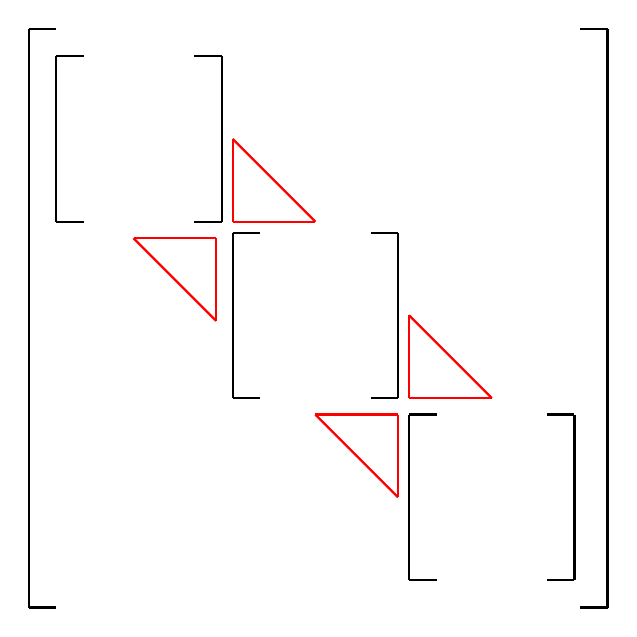
\begin{tikzpicture}[scale = 0.7]
\draw[thick] (0,10) -- (0,-0.5);
\draw[thick] (0,10) -- (0.5,10);
\draw[thick] (0,-0.5) -- (0.5,-0.5);
\draw[thick] (10.5,10) -- (10.5,-0.5);
\draw[thick] (10.5,10) -- (10,10);
\draw[thick] (10,-0.5) -- (10.5,-0.5);
\draw[thick] (0.5,9.5) -- (0.5,6.5);
\draw[thick] (0.5,9.5) -- (1,9.5);
\draw[thick] (0.5,6.5) -- (1,6.5);
\draw[thick] (3.5,9.5) -- (3,9.5);
\draw[thick] (3.5,6.5) -- (3,6.5);
\draw[thick] (3.5,9.5) -- (3.5,6.5);
\draw[thick] (3.7,6.3) -- (3.7,3.3);
\draw[thick] (6.7,6.3) -- (6.7,3.3);
\draw[thick] (3.7,6.3) -- (4.2,6.3);
\draw[thick] (3.7,3.3) -- (4.2,3.3);
\draw[thick] (6.7,3.3) -- (6.2,3.3);
\draw[thick] (6.7,6.3) -- (6.2,6.3);
\draw[thick] (6.9,3) -- (6.9,0);
\draw[thick] (6.9,3) -- (7.4,3);
\draw[thick] (6.9,0) -- (7.4,0);
\draw[thick] (9.9,3) -- (9.9,0);
\draw[thick] (9.9,3) -- (9.4,3);
\draw[thick] (9.9,0) -- (9.4,0);



\draw[thick,red] (3.7,6.5) -- (3.7,8);
\draw[thick,red] (3.7,6.5) -- (5.2,6.5);
\draw[thick,red] (3.7,8) -- (5.2,6.5);

\draw[thick,red] (6.9,3.3) -- (6.9,4.8);
\draw[thick,red] (6.9,3.3) -- (8.4,3.3);
\draw[thick,red] (6.9,4.8) -- (8.4,3.3);

\draw[thick,red] (6.7,3) -- (6.7,1.5);
\draw[thick,red] (6.7,3) -- (5.2,3);
\draw[thick,red] (5.2,3) -- (6.7,1.5);

\draw[thick,red] (3.4,6.2) -- (3.4,4.7);
\draw[thick,red] (3.4,6.2) -- (1.9,6.2);
\draw[thick,red] (1.9,6.2) -- (3.4,4.7);

\end{tikzpicture}
\end{center}
}
\frame{
\begin{center}
\begin{tikzpicture}[scale = 0.7]
\draw[thick] (0,10) -- (0,-0.5);
\draw[thick] (0,10) -- (0.5,10);
\draw[thick] (0,-0.5) -- (0.5,-0.5);
\draw[thick] (10.5,10) -- (10.5,-0.5);
\draw[thick] (10.5,10) -- (10,10);
\draw[thick] (10,-0.5) -- (10.5,-0.5);
\draw[thick] (0.5,9.5) -- (0.5,6.5);
\draw[thick] (0.5,9.5) -- (1,9.5);
\draw[thick] (0.5,6.5) -- (1,6.5);
\draw[thick] (3.5,9.5) -- (3,9.5);
\draw[thick] (3.5,6.5) -- (3,6.5);
\draw[thick] (3.5,9.5) -- (3.5,6.5);
\draw[thick] (3.7,6.3) -- (3.7,3.3);
\draw[thick] (6.7,6.3) -- (6.7,3.3);
\draw[thick] (3.7,6.3) -- (4.2,6.3);
\draw[thick] (3.7,3.3) -- (4.2,3.3);
\draw[thick] (6.7,3.3) -- (6.2,3.3);
\draw[thick] (6.7,6.3) -- (6.2,6.3);
\draw[thick] (6.9,3) -- (6.9,0);
\draw[thick] (6.9,3) -- (7.4,3);
\draw[thick] (6.9,0) -- (7.4,0);
\draw[thick] (9.9,3) -- (9.9,0);
\draw[thick] (9.9,3) -- (9.4,3);
\draw[thick] (9.9,0) -- (9.4,0);

\draw[dashed] (2,8.2) -- (2,5.2);
\draw[dashed] (2,8.2) -- (2.5,8.2);
\draw[dashed] (2,5.2) -- (2.5,5.2);
\draw[dashed] (5,8.2) -- (5,5.2);
\draw[dashed] (5,5.2) -- (4.5,5.2);
\draw[dashed] (5,8.2) -- (4.5,8.2);

\draw[dashed] (5.2,4.9) -- (5.2,1.9);
\draw[dashed] (5.2,4.9) -- (5.7,4.9);
\draw[dashed] (5.2,1.9) -- (5.7,1.9);
\draw[dashed] (8.2,4.9) -- (8.2,1.9);
\draw[dashed] (8.2,4.9) -- (7.7,4.9);
\draw[dashed] (8.2,1.9) -- (7.7,1.9);



\end{tikzpicture}
\end{center}
}

\frame{
\frametitle{Erste Veruche/Probleme }
\begin{itemize}
\item
Original und Aufteilung waren fast immer gleich schnell
\item
Anfangs wurde bei jedem Schritt die Teilmatrix genormt
\item
Dies führte dazu das die Eigenvektoren falsch korrigiert wurden
\end{itemize}
}

\frame{
  \begin{center}
  \begin{tikzpicture}
  \node[rectangle,fill=blue!20,draw=blue!50,ultra
  thick,align=center,rounded corners=3mm] (matrix) {pseudo Google
    Matrix generieren};

  % ganze Matrix
  \node[below=of matrix,xshift=-1cm] (original){};
  \node at (original){n};
  \draw[->,>=stealth',very thick,green!40!black](original) ++(-175:.3cm) 
    arc (-175:120:.3cm) --++ (195:.1cm);
  \node[left=of original,xshift=.5cm,align=left] {Gesamt\\ mit Normierung};

  % Teilmatrix
  \node[below=of matrix,xshift=1cm] (teil10) {};
  \node at (teil10){10};
  \draw[->,>=stealth',very thick,blue!50!black] (teil10) ++(-175:.3cm)
    arc (-175:120:.3cm) --++ (195:.1cm);
  \node[right=of teil10,xshift=-.5cm,align=left] {Teil\\ ohne Normierung};

  \node[below=of teil10] (gesamt1) {};
  \node at (gesamt1) {1};
  \draw[->,>=stealth',very thick,brown!40!black] (gesamt1) ++ (-175:.3cm)
    arc (-175:120:.3cm) --++ (195:.1cm);
  \node[right=of gesamt1,xshift=-.5cm,align=left] {Gesamt\\ mit Normierung};

  \node[below=of gesamt1] (teilN) {};
  \node at (teilN) {n};
  \draw[->,>=stealth',very thick,orange!80!black] (teilN) ++ (-175:.3cm)
    arc (-175:120:.3cm) --++ (195:.1cm);
  \node[right=of teilN,xshift=-.5cm,align=left] {Teil\\ ohne Normierung};

  \node[below=of teilN] (gesamtN) {};
  \node at (gesamtN) {n};
  \draw[->,>=stealth',very thick,green!40!black] (gesamtN) ++ (-175:.3cm)
    arc (-175:120:.3cm) --++ (195:.1cm);
  \node[right=of gesamtN,xshift=-.5cm,align=left] {Gesamt\\ mit Normierung};

  % Verbindungen
  \draw[->,>=stealth',thick,shorten >=.3cm,shorten <=.4cm] (matrix) ++
    (180:1cm) to (original);

  \draw[->,>=stealth',thick,shorten >=.3cm,shorten <=.4cm] (matrix) ++
    (0:1cm) to (teil10);
  \draw[->,>=stealth',thick,shorten >=.3cm,shorten <=.3cm] (teil10) to
    (gesamt1);
  \draw[->,>=stealth',thick,shorten >=.3cm,shorten <=.3cm] (gesamt1) to
    (teilN);
  \draw[->,>=stealth',thick,shorten >=.3cm,shorten <=.3cm] (teilN) to
    (gesamtN);
  \end{tikzpicture}
  \end{center}
}

\frame{
\frametitle{Ausgabe des Codes}
\renewcommand{\arraystretch}{1.4}
\begin{center}

\begin{tabular}{|l|c|c|c|}
\hline
 & $10^2x10^2$ & $10^3x10^3$ & $10^4x10^4$ \\
 \hline
Zeit Original & 0.179 &  18.063& 1667.8 \\
Eigenwert Original & 1.00 & 1.00  & 1.00\\
Schritte Original & 1572 & 9305 &  10782\\
global Norm & 13.604 & 42.850 &  137.220\\
global Norm & 1.08 & 1.014 &  1.013\\ 
global Norm & 1.07 & 1.012  & 1.012 \\
Zeit Bearbeitet & 0.948 & 5.088 &  442.81\\
Eigenwert Bearbeitet & 1.00 & 1.00  & 1.00 \\
Schritte Bearbeitet & 4 & 27 &  461\\
Teilmatrix Grösse & 50 & 500 & 5000 \\
\hline
\end{tabular}
\end{center}
}

\frame
{
\frametitle{Beispiel aus Code}
\begin{minipage}{0.48\textwidth}
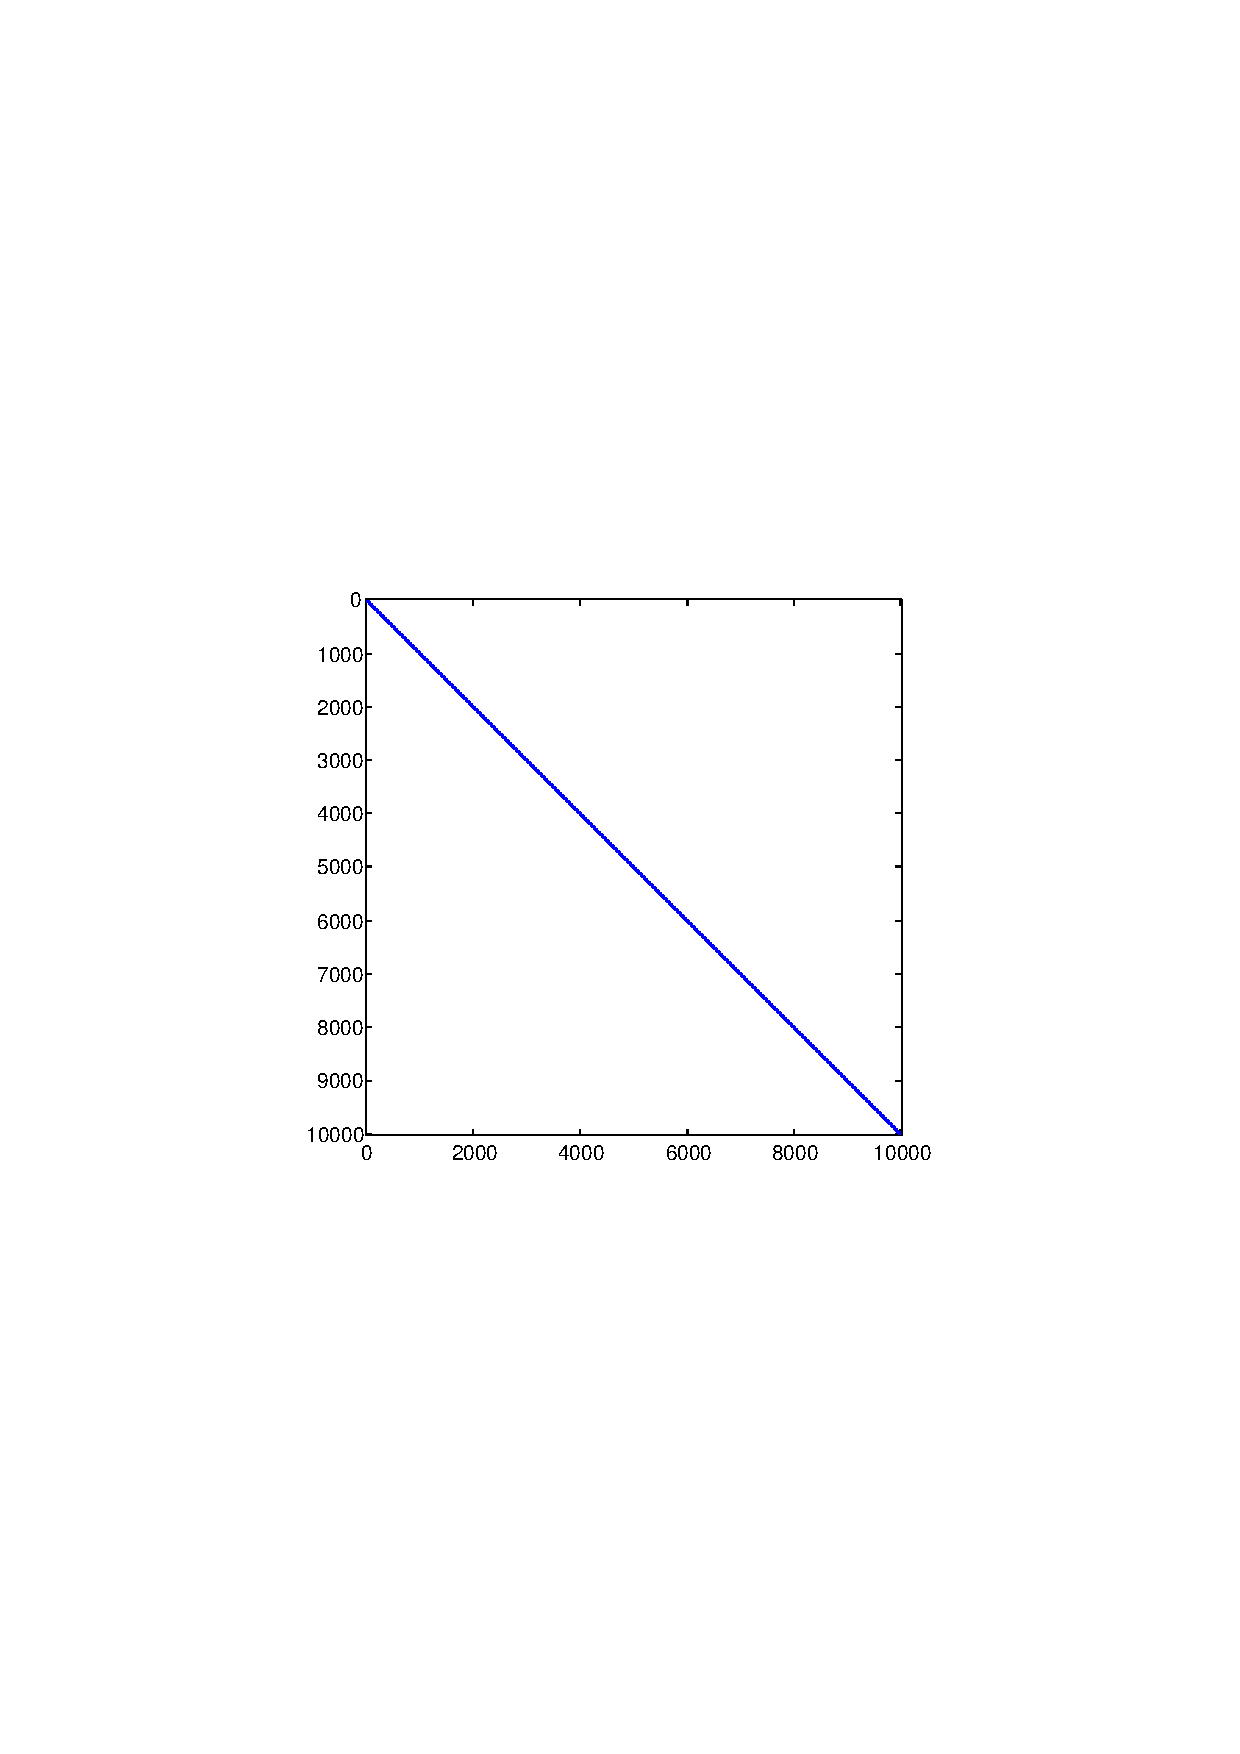
\includegraphics[width=0.9\textwidth]{./Bilder/spy}
\end{minipage}
\hspace{0.1cm}
\begin{minipage}{0.48\textwidth}
\lstinputlisting[breaklines=true]{GoogleMatrix.m}
\end{minipage}

}

\frame{
\begin{center}
\textbf{Parallelisierung der for Schlaufen}
\end{center}
\lstinputlisting[breaklines=true]{parfor.m}
}






\frame{
\frametitle{Auswertung der Berechnungszeiten}
\begin{itemize}
\item
Berechnungen von $10^2x10^2$, $10^3x10^3$, $10^4x10^4$ Matrizen
\item
Je 100 (5) Durchläufe mit unterschiedlichen random Google Matrizen
\item
Jeder der 100 (5) Durchläufe wird über die original Matrix und alle Teilmatrizen berechnet

\item
Trotz random Matrix erhalten wir gute Durchschnittswerte

\end{itemize}
}


\frame{
\begin{center}
 \includegraphics[width= 0.8\textwidth]{./bilder/PC100.pdf}
\end{center}

}
\frame{
\begin{center}
 \includegraphics[width= 0.8\textwidth]{./bilder/PC1000.pdf}
\end{center}
}

\frame{
\begin{center}
 \includegraphics[width= 0.8\textwidth]{./bilder/PC10000.pdf}
\end{center}
}

\frame{
\begin{center}
\begin{minipage}{0.5\textheight}
\includegraphics[width=\textwidth,page=1]{./bilder/PC3.pdf}
\end{minipage}
\\
\begin{minipage}{0.5\textheight}
\includegraphics[width=\textwidth,page=2]{./bilder/PC3.pdf}
\end{minipage}
\begin{minipage}{0.5\textheight}
\includegraphics[width=\textwidth,page=3]{./bilder/PC3.pdf}
\end{minipage}
\end{center}
}

\frame{
\frametitle{Berechnungszeitgewinn der besten Methode}
\renewcommand{\arraystretch}{1.4}
\begin{center}
\begin{tabular}{|c|c|c|}
\hline
Matrix & Teilmatrizen & In \% von der Originalzeit \\
\hline
1000 x 1000 & 250  &  50.68\%

\\
1000 x 1000 & 200  &  53.97\%
  \\
1000 x 1000 & 125  &  62.89\%
 \\
10000 x 10000 & 1000 &  22.93\% \\
10000 x 10000  & 100 & 25.12\%  \\
10000 x 10000 & 500 &  27.22\% \\
\hline
\end{tabular}
\end{center}
}

\frame{
\begin{center}
\includegraphics[width=0.8\textwidth]{./bilder/Ver.pdf}
\end{center}
}




%%% Local Variables: 
%%% mode: latex
%%% TeX-master: "main"
%%% End: 

% % % djkasdgjkaedrkbgnjfneanlglne

